\chapter{Informative Seafloor Exploration}
\lhead{Informative Seafloor Exploration}
\label{InformativeSeafloorExploration}

	The Gaussian process based inference model for benthic habitat mapping devised in Chapter \ref{BenthicHabitatMapping} provides a Bayesian framework for habitat inference and prediction. With such an inference model, this chapter proceeds to develop an informative path planning policy for benthic habitat mapping.
	
	In order to devise an informative path planning policy, it is important to select an appropriate acquisition criterion which measures the desirability of traversing a particular candidate path. Section \ref{Background:RelatedWork} provided an outline of related investigations on various acquisition functions for informative path planning in the benthic habitat mapping context, which motivated the need for a measure of mutual information. Such a measure would allow inference based on the \textit{essential} information contained in any given sub-region of interest. The mutual information criterion can then be employed as the acquisition function for informative path planning, in order to evaluate thus compare the desirability of visiting candidate regions and locations.
	
	Nevertheless, as Gaussian process classifiers lack analytical forms for the predictive joint distribution of target labels, any mutual information measure derived from the predictive joint distribution must rely on numerical estimation techniques. As such, estimating joint prediction information entropy requires a Monte Carlo sampling based approach. Section \ref{InformativeSeafloorExploration:MCJPIE} describes such a mutual information criterion, hereby named Monte Carlo Predictive Information Entropy (MCPIE).
	
	However, a Monte Carlo approach suffers some several drawbacks, such as computational complexity and limited estimation accuracy. Instead, this thesis proposes a new and alternative mutual information measure, Linearised Model Differential Entropy (LMDE), that is more computationally tractable than MCPIE. Section \ref{InformativeSeafloorExploration:LMDE} defines and derives LMDE as an appropriate form of mutual information. Specifically, it regularises between reducing mutual bias and mutual uncertainty through taking advantage of both the latent mean and covariance structure, as well as the non-Gaussian likelihood response. Tractability of the approach is further improved through a linearisation approximation on such an acquisition criterion.
	
	Section \ref{InformativeSeafloorExploration:ComparisonMutualEntropyMeasures} proceeds to demonstrate the two mutual entropy measures through example datasets. Interpretation of the experimental results provides an intuitive understanding of their differences in time complexity, accuracy, and most importantly, their properties.
	
	Section \ref{InformativeSeafloorExploration:RecedingHorizonFormulation} then formulates a receding horizon approach to informative path planning. This provides a simple yet effective framework for a large scale exploration task such as seafloor exploration for benthic habitat mapping. In particular, the receding horizon formulation strikes a balance between exploring in a non-myopic way and doing so with reasonable tractability constraints.
	
	Finally, section \ref{InformativeSeafloorExploration:ScottReef} assesses the performance of various approaches to informative seafloor exploration for benthic habitat mapping. Multiple acquisition criterions are tested under both the receding horizon approach and a myopic greedy approach, which verifies the benefits of linearised model differential entropy under the receding horizon formulation. Under a mapping accuracy criterion, simulations over the Scott Reef dataset demonstrates that LMDE acquisition outperform other criterions, including MCJPIE acquisition.
		
	\section{Monte Carlo Predictive Information Entropy}
	\label{InformativeSeafloorExploration:MCJPIE}
	
		This section introduces the Monte Carlo predictive information entropy (MCPIE) of Gaussian process classifiers. Monte Carlo sampling methods provide a way to estimate the joint predictive entropy through considering the joint distributions of the latent function at the query points.
	
		Monte Carlo sampling, as its name suggests, involve using sampled draws from a particular distribution to estimate a certain quantity that can be characterised by the distribution. In MCPIE case, the distribution to be sampled from is the latent GP process of the GP classifier, whose moments are analytically tractable, and the quantity to be estimated is the predictive information entropy of the query points. A brief description of the method is provided for both binary and multiclass classification.
		
		\subsection{Binary Classification}
		\label{InformativeSeafloorExploration:MCJPIE:Binary}
		
			Suppose a Gaussian process classifier has been trained under Laplace approximation with respect to a training set $\mathcal{D} = \{X, \bvec{y}\} = \{[ \bvec{x}_{1}, \bvec{x}_{2}, \dots, \bvec{x}_{n}]^{T}, [y_{1}, y_{2}, \dots, y_{n}]^{T}\}$ with $n$ training points. It is known that the latent function $f(\bvec{x})$ is distributed as a GP with a particular predictive mean $m(\bvec{x})$ and covariance $k(\bvec{x}, \bvec{x}')$ once conditioned on the training data \eqref{Equation:PredictiveLatentBinaryGP}. Note that again this section will omit explicitly notating the training data and query data that was conditioned upon. \begin{equation}
				f(\bvec{x}) \sim \mathcal{GP}(m(\bvec{x}), k(\bvec{x}, \bvec{x}'))
			\label{Equation:PredictiveLatentBinaryGP}
			\end{equation}
			
			Let $X^{\star} = [ \bvec{x}^{\star}_{1}, \bvec{x}^{\star}_{2}, \dots, \bvec{x}^{\star}_{n^{\star}}]^{T}$ denote the collection of $n^{\star}$ query points for which inference is to be performed upon. Denote $\bvec{f}^{\star}$ the vector of latent function values $f^{\star}_{i} = f(\bvec{x}^{\star}_{i})$ at each query point. By definition of a GP, $\bvec{f}^{\star}$ is multivariate Gaussian distributed with corresponding means $\mu^{\star}_{i} = m(\bvec{x}^{\star}_{i})$ and covariances $\Sigma^{\star}_{ij} = k(\bvec{x}^{\star}_{i}, \bvec{x}^{\star}_{j})$ \eqref{Equation:BinaryPredictiveGaussianDistribution}. \begin{equation}
				\bvec{f}^{\star} = [f^{\star}_{1}, f^{\star}_{2}, \dots, f^{\star}_{n^{\star}}]^{T} \sim \mathcal{N}(\vec{\upmu}^{\star}, \Sigma^{\star})
			\label{Equation:BinaryPredictiveGaussianDistribution}
			\end{equation}
				
			The binary prediction probability $\vec{\uppi^{\star}}$ at the query points is obtained through passing the queried latent function random vector $\bvec{f}^{\star}$ through a response function in a component wise fashion \eqref{Equation:PredictiveResponse}. \begin{equation}
				\vec{\uppi}^{\star} = \vec{\upsigma}(\bvec{f}^{\star})\mathrm{ \quad i.e. \;\;}\pi^{\star}_{i} = \sigma(f^{\star}_{i}) \quad \forall i \in I_{n^{\star}}
			\label{Equation:PredictiveResponse}
			\end{equation}
			
			As a straightforward transformation of the latent vector, the predictive probability vector $\vec{\uppi^{\star}}$ is thus a random vector itself. The usual procedure is then to treat the expected prediction probabilities $\mathbb{E}[\vec{\uppi^{\star}}]$ as the posterior class probabilities for further inference. However, this discards any information regarding the joint behaviour of an arbitrary collection of query points. As a result, a measure of mutual information shared amongst the query points cannot be obtained.
			
			As such, one straightforward approach to address this problem is to perform Monte Carlo estimation of the posterior joint distribution for class predictions via jointly sampling latent vectors from the GP latent, whose distribution is completely characterised through \eqref{Equation:PredictiveLatentBinaryGP} and definition \ref{Definition:GaussianRandomField}. For each jointly sampled vector, the components with positive latent values are assigned class label 1, and -1 otherwise. That is, for a particular sample ${^{s}}\bvec{f}^{\star}$ drawn from $\bvec{f}^{\star} \sim \mathcal{N}(\vec{\upmu}^{\star}, \Sigma^{\star})$ \eqref{Equation:BinaryPredictiveGaussianDistribution}, $s \in I_{n_{S}}$ where $n_{S}$ is the number of samples, the corresponding class assignments are computed through \eqref{Equation:MonteCarloSamplingBinaryClassifier}. Here, the left superscript $s$ indexes the sampled value or vector. As before, without the left superscript $s$, $\bvec{f}^{\star}$ is a random vector, while ${^{s}}\bvec{f}^{\star}$ is a particular realised, fixed vector. \begin{equation}
				{^{s}}\bvec{y}^{\star} = \bvec{\mathds{H}}({^{s}}\bvec{f}^{\star}) := \{\mathbb{H}({^{s}}f^{\star}_{i})\}_{i \in I_{n^{\star}}} \quad \forall s \in I_{n_{s}} \quad \mathrm{where} \quad \mathbb{H}(z) := \mathds{1}_{z > 0} - \mathds{1}_{z \leq 0}
			\label{Equation:MonteCarloSamplingBinaryClassifier}
			\end{equation}
			
			where $\mathbb{H}(z)$ is the modified Heaviside function which is 1 is $z$ is positive and -1 otherwise, so that ${^{s}}\bvec{y}^{\star} \in \{-1, 1\}^{n_{S}}$. Note that the sampled labels can be determined completely from the sampled latent function as, once sampled, the latent function is no longer a random function. Hence, any positive (negative) latent values will map to prediction probabilities of more (less) than 0.5 under any likelihood response.
			
			Further, define $I_{U} \subseteq I_{n_{S}}$, $n_{U} := \Vert I_{U} \Vert$, as the indices corresponding to the subset with the maximum amount of unique samples \eqref{Equation:UniqueIndexSet}.
			
			\begin{equation}
				I_{U} := \argmax_{\{I \subseteq I_{n_{S}} | {^{s}}\bvec{y}^{\star} \neq {^{t}}\bvec{y}^{\star}, \forall s, t \in I\}} \Vert I \Vert 
			\label{Equation:UniqueIndexSet}
			\end{equation}			
			
			where $\Vert I \Vert$  stands for the cardinality of $I$. An \textit{estimated} probability vector $\tilde{\bvec{p}}$ can then be formed \eqref{Equation:EstimatedProbability}.

			\begin{equation}
				\begin{aligned}
					\tilde{\bvec{p}}^{\star} &:= \bigg\{ \frac{1}{n_{S}}\mathbb{F}_{I_{n_{S}}}({^{s}}\bvec{y}^{\star}) \bigg\}_{s \in I_{U}} \\
					\mathbb{F}_{I_{n_{S}}}({^{s}}\bvec{y}^{\star}) &:= \sum_{t \in I_{n_{S}}} \mathds{1}_{{^{s}}\bvec{y}^{\star} = {^{t}}\bvec{y}^{\star}}
				\end{aligned}
			\label{Equation:EstimatedProbability}
			\end{equation}
			
			where $\mathbb{F}_{I_{n_{S}}}({^{s}}\bvec{y}^{\star})$ is the frequency of appearance of the vector ${^{s}}\bvec{y}^{\star}$ amongst all the sampled vectors $\{ {^{s}}\bvec{y}^{\star} \}_{s \in I_{n_{S}}}$. Note that each \textit{unique} sample is assigned a probability such that the vector $\tilde{\bvec{p}}^{\star}$ has exactly $n_{U}$ non-zero entries indexed by $I_{U}$, which is generally smaller than the total number of possible samples. This inherently means that possible samples that were not drawn or \textit{realised} are estimated with probability zero. In this way, since more samples would likely realise those unlikely possibilities and thus raising the corresponding probability to a nonzero value, estimation accuracy will benefit from higher numbers of samples $n_{S}$.
			
			Finally,  for $n_{C} = 2$ classes, the Monte Carlo predictive information entropy, as an instance of Shannon entropy \eqref{Equation:DiscreteEntropy}, can be computed from the estimated probabilities that represent the joint distribution \eqref{Equation:MCPIE}. As usual, only non-zero entries of $\tilde{\bvec{p}}$ need to be considered. 
			
			\begin{equation}
				H_{\mathrm{MCPIE}} \stackrel{\text{abbrev.}}{:=} H_{\mathrm{MCPIE}}[X^{\star} | X, \bvec{y}] := - \sum_{i \in I_{n_{U}}} \tilde{p}^{\star}_{i} \log(\tilde{p}^{\star}_{i})
			\label{Equation:MCPIE}
			\end{equation}		
			
		\subsection{Multiclass Classification}
		\label{InformativeSeafloorExploration:MCJPIE:Multiclass}
		
			The derivation in the multiclass case is similar to the binary case. Specifically, since ${^{s}}\bvec{y}^{l} \in \{1, 2, \dots, n_{C}\}^{n_{s}}$ it suffices to replace the sampling step \eqref{Equation:MonteCarloSamplingBinaryClassifier} with \eqref{Equation:MonteCarloSamplingMulticlassClassifier}.
			
			The following sampling method assumes that the GP classifier has been trained under a OVA scheme (see section \ref{BenthicHabitatMapping:Classification:MulticlassClassification:OVA}). Analogous to \eqref{Equation:PredictiveLatentBinaryGP}, for $c$ classes, there are $n_{C}$ latent functions $\{f^{1}(x), f^{2}(x), \dots, f^{n_{C}}(x)\}$ corresponding to each class \eqref{Equation:PredictiveLatentMulticlassGP}. \begin{equation}
				f^{c}(\bvec{x}) \sim \mathcal{GP}(m^{c}(\bvec{x}), k^{c}(\bvec{x}, \bvec{x}')) \qquad \forall c \in I_{n_{C}}
			\label{Equation:PredictiveLatentMulticlassGP}
			\end{equation}
						
			Here the superscript $c$ is used to index the classes. The latent vector $\bvec{f}_{i} := \{f^{c}_{i}\}_{c \in I_{n_{C}}}$ represents the collection of $n_{C}$ latent values across classes at the query point $i \in I_{n^{\star}}$, and is distinct from $\bvec{f}^{c} := \{f^{c}_{i}\}_{i \in I_{n^{\star}}}$ which represents the collection of $n^{\star}$ latent values across query points for class $c \in I_{n_{C}}$.
			
			Again, by definition of a GP, each ${\bvec{f}^{c}}^{\star}$ is multivariate Gaussian distributed with corresponding means ${\mu^{c}}^{\star}_{i} = m^{c}(\bvec{x}^{\star}_{i})$ and covariances ${\Sigma^{c}}^{\star}_{ij} = k^{c}(\bvec{x}^{\star}_{i}, \bvec{x}^{\star}_{j})$ \eqref{Equation:MulticlassPredictiveGaussianDistribution}. \begin{equation}
				{\bvec{f}^{c}}^{\star} = [{f^{c}}^{\star}_{1}, {f^{c}}^{\star}_{2}, \dots, {f^{c}}^{\star}_{n^{\star}}]^{T} \sim \mathcal{N}({\vec{\upmu}^{c}}^{\star}, {\Sigma^{c}}^{\star})
			\label{Equation:MulticlassPredictiveGaussianDistribution}
			\end{equation}
			
			For each class $c$, a sample ${^{s}}{\bvec{f}^{c}}^{\star}$ is drawn from ${\bvec{f}^{c}}^{\star} \sim \mathcal{N}({\vec{\upmu}^{c}}^{\star}, {\Sigma^{c}}^{\star})$, where $s \in I_{n_{S}}$. The corresponding sampled target labels are then found by \eqref{Equation:MonteCarloSamplingMulticlassClassifier}. \begin{equation}
				\begin{aligned}
					{^{s}}\bvec{y}^{\star} = \bvec{\mathds{M}}_{n_{C}}({^{s}}{\bvec{f}^{1}}^{\star}, {^{s}}{\bvec{f}^{2}}^{\star}, \dots, {^{s}}{\bvec{f}^{n_{C}}}^{\star}) &:= \{\mathbb{M}_{n_{C}}({^{s}}{f^{1}}^{\star}_{i}, {^{s}}{f^{2}}^{\star}_{i}, \dots, {^{s}}{f^{n_{C}}}^{\star}_{i})\}_{i \in I_{n^{\star}}} \quad \forall s \in I_{n_{s}} \\
					\mathrm{where} \qquad \mathbb{M}_{n_{C}}(z_{1}, z_{2}, \dots, z_{n_{C}}) &:= \argmax_{c \in I_{n_{C}}} z_{c}
				\end{aligned}
			\label{Equation:MonteCarloSamplingMulticlassClassifier}
			\end{equation}
			
			That is, for each sample $s \in I_{n_{S}}$ and at each query point $i \in I_{n^{\star}}$, ${^{s}}y^{\star}_{i}$ is assigned the class label from $\{1, 2, \dots, n_{C}\}$ that has the maximal latent value. With the samples $\{{^{s}}\bvec{y}^{\star}\}_{s \in I_{n_{s}}}$, the estimated probability can be computed from \eqref{Equation:EstimatedProbability}, so that the Monte Carlo predictive information entropy for $n_{C} > 2$ classes can also be computed from \eqref{Equation:MCPIE}.
			
	\section{Linearised Model Differential Entropy}
	\label{InformativeSeafloorExploration:LMDE}
	
		This section introduces the linearised model differential entropy (LMDE) of Gaussian process classifiers. This method attempts to address the need for a measure of mutual entropy that is more computationally viable compared than Monte Carlo methods. Through investigating the structure of the GP classification inference model in both the binary and multiclass classification setting, a simple derivation for LMDE is provided.
		
		\subsection{Binary Classification}
		\label{InformativeSeafloorExploration:LMDE:Binary}
		
			For binary classification, linearisation is performed on the likelihood response.
					
			The beginning of this derivation is the same as section \ref{InformativeSeafloorExploration:MCJPIE:Binary} up to \eqref{Equation:PredictiveResponse}. At this stage, instead of proceeding with Monte Carlo sampling, it is proposed to use the joint distribution of the predictive probabilities $\vec{\uppi^{\star}}$ itself as a basis of constructing a measure of mutual information. Unlike traditional approaches where inference depends only on the expectance $\mathbb{E}[\vec{\uppi^{\star}}]$ such that structural information from the latent GP is compromised, it is aimed to utilise also the covariance $\mathbb{V}[\vec{\uppi^{\star}}]$, which contains information regarding both the latent GP and the response likelihood.
		
			\begin{figure}[!htbp]
				\centering
					\includegraphics[width = 0.6\linewidth]{Figures/linearisation.eps}
				\caption{Linearisation accuracy for a probit response: Green shade represents the latent variance while blue shade represents the predictive variance. Gold lines show local linearisation about latent expectance.}
				\label{Figure:Linearisation}
			\end{figure}
				
			As the predictive probabilities are nonlinear transformations of the Gaussian distributed latent vector, they are no longer Gaussian distributed. In order to retain analytical tractability, the proposed approach is to linearise the response function about the latent expectance $\bar{f}^{\star}_{i} := \mathbb{E}[f^{\star}_{i}]$. Figure \ref{Figure:Linearisation} illustrates the linearisation accuracy for a probit response. Observe that points with latent expectance far away from zero translate to near zero predictive variance even under high latent variance. Linearisation is thus very accurate for those points. For points with latent expectances near zero, we require the latent variances to be sufficiently small for linearisation to be accurate.
			
			The linearised can thus be derived, which also serves to construct the definition of linearised differential entropy. With first order Taylor expansion, the response is linearised the latent mean $\bar{f}^{\star}_{i} = \mathbb{E}[f^{\star}_{i}]$ \eqref{Equation:LinearisingSigmoid}. \begin{equation}
				\sigma(f^{\star}_{i}) \approx \sigma_{L}(f^{\star}_{i}) := \sigma(\bar{f}^{\star}_{i}) + \sigma'(\bar{f}^{\star}_{i}) (f^{\star}_{i} - \bar{f}^{\star}_{i})
			\label{Equation:LinearisingSigmoid}
			\end{equation}
			
			The prediction probabilities are now approximated as a linear transformation $\sigma_{L}(f)$ of the latent vector, so that it is also multivariate Gaussian distributed with expectance and covariance available in analytical form \eqref{Equation:MomentsLinearisedSigmoid}. \begin{align*}
			\numberthis \label{Equation:MomentsLinearisedSigmoid}
					\vec{\upsigma}_{L}(\bvec{f}^{\star}) & \sim \mathcal{N}(\vec{\upmu}^{\star}_{L}, \Sigma^{\star}_{L}) \\
					({\mu^{\star}_{L}})_{i} & = \mathbb{E}[\sigma_{L}(f^{\star}_{i})] = \sigma(\bar{f}^{\star}_{i}) \\
					({\Sigma^{\star}_{L}})_{ij} & = \mathbb{C}\mathrm{ov}[\sigma_{L}(f^{\star}_{i}), \sigma_{L}(f^{\star}_{j})] = \sigma'(\bar{f}^{\star}_{i}) \sigma'(\bar{f}^{\star}_{j}) \mathbb{C}\mathrm{ov}[f^{\star}_{i}, f^{\star}_{j}]
			\end{align*}
			
			Finally, the linearised model differential entropy $H_{\mathrm{LMDE}}$ at the query points $X^{\star}$ is defined to be the differential entropy corresponding to the random vector $\vec{\upsigma}_{L}(\bvec{f}^{\star})$. Since $\vec{\upsigma}_{L}(\bvec{f}^{\star})$ is multivariate Gaussian distributed, $H_{\mathrm{LMDE}}$ exhibits a closed form \eqref{Equation:BinaryLinearisedEntropy}. \begin{equation}
				H^{\mathrm{binary}}_{\mathrm{LMDE}} \stackrel{\text{abbrev.}}{:=} H^{\mathrm{binary}}_{\mathrm{LMDE}}[X^{\star} | X, \bvec{y}] := \frac{1}{2} \log\Big((2 \pi e)^{n^{\star}} \det(\Sigma^{\star}_{L})\Big)
			\label{Equation:BinaryLinearisedEntropy}
			\end{equation}			
						
		\subsection{Multiclass Classification}
		\label{InformativeSeafloorExploration:LMDE:Multiclass}
		
			For multiclass classification, linearisation is performed on the softmax function $\sigma^{c}$ which returns the corresponding predictive class probability $\vec{\uppi}^{c}$ for class $c \in I_{n_{C}} := \{1, 2, \dots, n_{C}\}$ \eqref{Equation:Softmax} \citep{GaussianProcessForMachineLearning}. \begin{equation}
				{\pi^{c}_{i}}^{\star} = \sigma^{c}({\bvec{f}_{i}}^{\star}) := \frac{\exp({f^{c}_{i}}^{\star})}{\sum_{m = 1}^{n_{C}} \exp({f^{m}_{i}}^{\star})} \qquad c \in I_{n_{C}}
			\label{Equation:Softmax}
			\end{equation}
			
			Again, OVA classifiers are employed, where each class is trained against all other classes independently with a binary classifier. For $c$ classes, $c$ binary classifiers are trained independently and also performs inference independently. The normalisation is then inherently captured in the softmax \eqref{Equation:Softmax}. This approach avoids the Monte Carlo sampling step in the inference stage of a typical GP multiclass classifier under Laplace Approximation \citep{GaussianProcessForMachineLearning}, and is thus faster in computational time. Note that this Monte Carlo sampling step avoided is separate to the one used in MCJIE. In essence, using OVA classifiers skip one Monte Carlo step, and using LMDE skips another Monte Carlo step through avoiding using MCPIE. Furthermore, because each classifier is trained independently, both the learning stage and the inference stage can be performed in parallel, further speeding up the process in a way that was not available under the original scheme. This is important later in under a receding horizon formulation, where the inference stage is included in the objective function of an optimiser such that repeated evaluations would benefit dramatically from shorter inference time.
			
			Similar to the binary case, to linearise it is imperative to examine the gradient of each of the $c$ softmax functions \eqref{Equation:SoftmaxGradient}. For notational simplicity, the query stars ($^{\star}$) are omitted in this derivation except for $n^{\star}$.
			
			\begin{equation}
				\frac{\partial \sigma^{c}}{\partial f^{k}_{i}}(\bvec{f}_{i}) =
				\begin{cases} 
					- \frac{\exp(f^{c}_{i}) \exp(f^{k}_{i})}{\sum_{m = 1}^{n_{C}} \exp({f^{c}_{i}})} & \text{for } k \neq c  \\
					- \frac{\exp(f^{c}_{i})^{2}}{\big(\sum_{m = 1}^{n_{C}} \exp({f^{c}_{i}})\big)^{2}} + \frac{\exp(f^{c}_{i})}{\sum_{m = 1}^{n_{C}} \exp({f^{c}_{i}})}& \text{for } k = c
				\end{cases}
			\label{Equation:SoftmaxGradient}
			\end{equation}			
		
			The numerators are explicitly left in the form of products of exponentiation instead of exponentiation of sums to reflect ways to cache quantities during computation. 
			
			Hence, for each class $c$ at query point $i$ a softmax gradient vector is computed \eqref{Equation:SoftmaxGradientVector}.
			
			\begin{equation}
				\frac{\partial \sigma^{c}}{\partial \bvec{f}_{i}}(\bvec{f}_{i}) := \begin{bmatrix} \frac{\partial \sigma^{c}}{\partial f^{1}_{i}}(\bvec{f}_{i}) & \frac{\partial \sigma^{c}}{\partial f^{2}_{i}}(\bvec{f}_{i}) & \dots & \frac{\partial \sigma^{c}}{\partial f^{n_{C}}_{i}}(\bvec{f}_{i}) \end{bmatrix}^{T}
			\label{Equation:SoftmaxGradientVector}
			\end{equation}
			
			The linearisation is again performed on the mean latent predictions $\bar{\bvec{f}}_{i} = \mathbb{E}[\bvec{f}_{i}]$ so that each softmax $\sigma^{c}(\bvec{f}_{i})$ can be approximated with the linearised softmax $\sigma^{c}_{L}(\bvec{f}_{i})$ \eqref{Equation:LinearisedSoftmax} in an analogous form as \eqref{Equation:LinearisingSigmoid}.
			
			\begin{equation}
				\begin{aligned}
					\sigma^{c}(\bvec{f}_{i}) \approx \sigma^{c}_{L}(\bvec{f}_{i}) & := \sigma^{c}(\bar{\bvec{f}}_{i}) + \left. \frac{\partial \sigma^{c}}{\partial \bvec{f}_{i}} \right|^{T}_{\bvec{f}_{i} = \bar{\bvec{f}}_{i}} (\bvec{f}_{i} - \bar{\bvec{f}}_{i}) \\
					& = \bvec{a}^{c}_{i} + (\bvec{g}^{c}_{i})^{T} (\bvec{f}_{i} - \bar{\bvec{f}}_{i})
				\end{aligned}
			\label{Equation:LinearisedSoftmax}
			\end{equation}
			
			where we have notated the constants $\bvec{a}^{c}_{i} := \sigma^{c}(\bar{\bvec{f}}_{i})$ and $\bvec{g}^{c}_{i} := \frac{\partial \sigma^{c}}{\partial \bvec{f}_{i}}(\bar{\bvec{f}}_{i})$.
			
			To determine the distribution of the vector of softmax values across query points, first define the following \eqref{Equation:Definitions}.
			
			\begin{equation}
				\begin{aligned}
					F &:= \{f^{c}_{i}\}_{c \in I_{n_{C}}, i \in I_{n^{\star}}} \in \mathbb{R}^{n_{C} \times n^{\star}} \\
					\vec{\upsigma}^{c}_{L}(F) &:= \begin{bmatrix} \sigma^{c}_{L}(\bvec{f}_{1}) & \sigma^{c}_{L}(\bvec{f}_{2}) & \dots & \sigma^{c}_{L}(\bvec{f}_{n^{\star}}) \end{bmatrix}^{T} \qquad \forall c \in I_{n_{C}}
				\end{aligned}
			\label{Equation:Definitions}
			\end{equation}
						
			The covariance of the linearised softmax of a particular class $c$ between two query points $i$ and $j$ can now be computed, as well as the expectance at a particular query point $i$ \eqref{Equation:MomentsLinearisedSoftmax}.
			
			\begin{align*}
			\numberthis \label{Equation:MomentsLinearisedSoftmax}
					\vec{\upsigma}^{c}_{L}(F) & \sim \mathcal{N}(\vec{\upmu}^{c}_{L}, \Sigma^{c}_{L}) \\
					(\mu^{c}_{L})_{i} & = \mathbb{E}[\sigma^{c}_{L}(\bvec{f}_{i})] =  \sigma^{c}(\bar{\bvec{f}}_{i}) \\
					(\Sigma^{c}_{L})_{ij} & = \mathbb{C}\mathrm{ov}[\sigma^{c}_{L}(\bvec{f}_{i}), \sigma^{c}_{L}(\bvec{f}_{i})] \\
					& = \mathbb{C}\mathrm{ov}[(\bvec{g}^{c}_{i})^{T} \bvec{f}_{i}, (\bvec{g}^{c}_{j})^{T} \bvec{f}_{j}] \\
					& = \sum_{m = 1}^{n_{C}} (g^{c}_{i})^{m} (g^{c}_{j})^{m} \mathbb{C}\mathrm{ov}[f^{m}_{i}, f^{m}_{j}]
			\end{align*}
						
			where $(g^{c}_{i})^{m}$ denotes the $m^{\text{th}}$ element of $\bvec{g}^{c}_{i}$. The last equality arises as a result of employing OVA multiclass classification, where latent values of classes $c$ and $m$, $c \neq m$, are conditionally independent given training observations.
			
			Finally, the linearised entropy of the OVA multiclass Gaussian process classifier is defined as follows \eqref{Equation:MulticlassLinearisedEntropy}.
			
			\begin{equation}
				H^{\mathrm{multiclass}}_{\mathrm{LMDE}} \stackrel{\text{abbrev.}}{:=} H^{\mathrm{multiclass}}_{\mathrm{LMDE}}[X^{\star} | X, \bvec{y}] := \frac{1}{2} \log\Bigg((2 \pi e)^{n^{\star}} \det\bigg(\sum_{c = 1}^{n_{C}} \Sigma^{c}_{L}\bigg)\Bigg)
			\label{Equation:MulticlassLinearisedEntropy}
			\end{equation}			
		
	\section{Comparison of Mutual Entropy Measures}
	\label{InformativeSeafloorExploration:ComparisonMutualEntropyMeasures}
	
		Both Monte Carlo prediction information entropy and linearised model differential entropy are suitable measures of mutual entropy that can be used as an acquisition criterion for informative path planning. This section provides a simple comparison between the two entropy measures with example datasets, which would further assist in the interpretation of model differential entropy. The main takeaway is that MCPIE and LMDE are complementary measures of entropy which together captures uncertainty in prediction and uncertainty in the model respectively.
	
		\subsection{Estimation Accuracy under Monte Carlo Sampling}
		
			It is helpful to visualise the practical numbers of samples required for reasonable estimation accuracy for MCPIE. Figure \ref{Figure:mcpie_lmde_comparison_binary} shows a simple case for a binary classification scenario, while Figure \ref{Figure:mcpie_lmde_comparison_multiclass} shows a case for a multiclass classification scenario with 4 classes. 
			
			\begin{figure}[!htbp]
				\centering
					\includegraphics[width = \linewidth]{Figures/mcpie_lmde_comparison_binary/mcpie_lmde_comparison.eps}
				\caption{GP binary classifier example}
				\label{Figure:mcpie_lmde_comparison_binary}
			\end{figure}			
						
			In both cases, the training data are evenly distributed in the feature space with features $x_{1}$ and $x_{2}$. In both Figure \ref{Figure:mcpie_lmde_comparison_binary} and \ref{Figure:mcpie_lmde_comparison_multiclass}, the MCPIEs are estimated with 2500 samples \textit{at each query point}. Note that only the marginalised entropies can visualised, as it is difficult to visualise multiple regional entropies. However, this is sufficient to provide an intuition for the accuracy of the method.
			
			\begin{figure}[!htbp]
				\centering
					\includegraphics[width = \linewidth]{Figures/mcpie_lmde_comparison_multiclass/mcpie_lmde_comparison.eps}
				\caption{GP multiclass classifier example}
				\label{Figure:mcpie_lmde_comparison_multiclass}
			\end{figure}
			
			Since only the marginalised entropies are visualised, there exists analytical forms for prediction information entropy by computing the Shannon entropy over the expected prediction probabilities at each query point. For a multiclass case under the OVA formulation, the probabilities are fused using the \textit{exclusion} method (see section  \ref{Background:GaussianProcesses:Classification:OVA}). Subplots (2, 1) and (2, 2) of Figures \ref{Figure:mcpie_lmde_comparison_binary} and \ref{Figure:mcpie_lmde_comparison_multiclass} show the analytically computed PIE and Monte Carlo estimated PIE (MCPIE) respectively. Both cases show that with 2500 samples, the estimation is fairly accurate.
			
			\begin{figure}[!htbp]
				\centering
					\includegraphics[width = \linewidth]{Figures/mcpie_lmde_comparison_binary/mcpie_accuracy.eps}
				\caption{Accuracy improvement of MCPIE for a binary classification case}
				\label{Figure:mcpie_accuracy_binary}
			\end{figure}
				
			Figures \ref{Figure:mcpie_accuracy_binary} and \ref{Figure:mcpie_accuracy_multiclass} visualises the accuracy improvement as more samples are used for entropy estimation in the corresponding binary and multiclass case respectively. With low numbers of samples, the estimation is noisy and inaccurate, and generally converges to a reasonable accuracy after 1000 samples. Notice however that even with low numbers of samples, the entropies are mostly in the correct range already.
			
			\begin{figure}[!htbp]
				\centering
					\includegraphics[width = \linewidth]{Figures/mcpie_lmde_comparison_multiclass/mcpie_accuracy.eps}
				\caption{Accuracy improvement of MCPIE for a multiclass classification case}
				\label{Figure:mcpie_accuracy_multiclass}
			\end{figure}
			
		\subsection{Interpretation of Model Differential Entropy}
		\label{InformativeSeafloorExploration:LMDE:Interpretation}
		
			It is worthwhile to remember that linearised model differential entropy is not an approximation to the usual prediction information entropy - the former is a differential entropy on a multivariate Gaussian distribution and the latter is an information entropy on the distribution of discrete class predictions combinations, which is a multivariate multinomial distribution. They have different interpretations and both can have advantageous properties under different scenarios. It is proposed that using linearised model differential entropy as an alternative acquisition function for informative path planning can be more beneficial under specific exploration purposes.
			
			Specifically, while the prediction information entropy (PIE) represents the confidence in the model, the model differential entropy (MDE) represents the the separability of classes in the feature space. In fact, MDE quantifies the ambiguity of the predictive probabilities. In particular, it is possible for GP multiclass classifiers to conclude low predictive variance even under uncertain predictive probabilities. In this case, the MDE would be high while the PIE would be low at such locations, indicating that the model is confident about its inability to separate classes \citep{AsherBender}. Similar to the bias-variance trade-off, such a situation indicate high bias, and is distinct from a model that is unconfident about its ability to separate classes, which would correspond to high variance. In fact, as the entropy of the prediction probabilities, model differential entropy is so named as it measures the uncertainty in the model itself. While an uncertainty in the model propagates into uncertainty in the prediction, it also propagates into bias in the prediction as an inaccurate model is unlikely to predict the correct class labels on average. This demonstrates that PIE and MDE are two complementary measures of entropy that can assist each other in identifying both places of high bias and high variance.
			
			In this way, using MDE as the acquisition function means that the vehicle would prioritise on both getting the both the model and predictions as correct as possible, instead of only focusing on predictions as in the PIE case.
			
		\subsection{Advantage of Model Differential Entropy}
		
			Here the examples from Figures \ref{Figure:mcpie_lmde_comparison_binary} and \ref{Figure:mcpie_lmde_comparison_multiclass} are discussed further in detail.
			
			With abundant and evenly distributed training data, the classifiers achieves a misclassification rate of only 2.2\% and 8.6\% respectively. The classifiers are trained with an axis aligned Gaussian kernel with a probit response under Laplace approximation. 
			
			Intuitively, under abundant data, it is desired that the classifier would only indicate high entropies at decision boundaries. In Figure \ref{Figure:mcpie_lmde_comparison_binary}, the prediction information entropy is indeed near its maximum at the predicted decision boundaries. As an artefact of the Laplace approximation, however, it is also quite high around the edges where the classifier has learned a slightly lower signal to noise ratio. In this example, there are no training points around the edges shown. As a result, the GP classifier learns a slightly lower signal to noise ratio in the latent function, and bounces back to its latent GP prior for which it remains uncertain regarding class label assignments. The prediction information entropy reflects this change more rapidly, so that it is high both at the decision boundaries and wherever observations are lacking. If the acquisition function for informative exploration is a function of the prediction information entropy, the vehicle would be suggested to explore both places with lacking observations and the decision boundaries. 
	
			This leads to the classic exploration-exploitation dilemma most machine learning algorithms face. It is possible that there exists decision boundaries yet to be detected at regions of lower relative data density. Is it worth it for the vehicle to explore and discover such regions, or exploit the currently known boundaries and map it better? In most exploration applications, the priority is to map the region of interest as accurately and fast as possible in order to reduce time and cost. While it is possible that there exists undiscovered decision boundaries at regions of lower relative data density, it is undesirable under cost constraints that this possibility is weighed heavily by the vehicle even under abundant data.
					
			On the other hand, linearised model differential entropy focuses on the decision boundary as it is constructed to be only high when the latent function is near zero (figure \ref{Figure:Linearisation}). Figure \ref{Figure:mcpie_lmde_comparison_binary} shows that that LMDE emphasizes on where the latent expectance is close to zero, and filters out the rest. If LMDE is used as the acquisition function, the vehicle would focus on the decision boundaries within the feature space, so that the vehicle would focus strictly on the mapping the predicted decision boundaries better. Notice that regions far away from observations in the feature space are also assigned with high linearised differential entropy, as the latent function bounces back to its prior, so that the vehicle would explore those parts of the feature space if necessary.
			
			Figure \ref{Figure:mcpie_lmde_comparison_multiclass} shows a similar scenario with a multi-class scenario with 4 labels. The same behaviour as the binary case is observed, where the LMDE approach pushes down the entropy level of all regions except the predicted decision boundaries.

			Furthermore, in the case of a feature space that does not contain the spatial coordinates for which path planning in based on, the MCPIE method may spent a lot of time in a single region where it is locally rich in span of a subspace of the feature space. However, this is suboptimal as this means it is giving up on trying to go for other regions that may have an even richer span of the feature space. The linearised model differential entropy method focuses its efforts (prioritises) the decision boundaries in the feature space at the expense of overlooking regions with less observations. This leads to smoother paths as it will look at all elements of the feature space. As long as one of the features is spatially correlated (depth in the benthic habitat mapping case), this will lead to smoother paths.
	
% 62500 QUERIES [MARGINALISED]
	
% BINARY 1: INFO:root:{'time_mcpie_high': 18.39458680280154, 'time_mcpie_med': 2.383764856014338, 'time_lmde': 0.009482532012810907, 'time_mcpie_low': 1.3273178461480555, 'time_pie': 0.0020675683150006563}

% MULTICLASS 1: INFO:root:{'time_mcpie_low': 2.2666649940613013, 'time_pie': 0.0048935111084738026, 'time_mcpie_med': 14.068846717692534, 'time_lmde': 0.18608571000102003, 'time_mcpie_high': 161.86858168576953}

% 30 QUERIES [MUTUAL]

% BINARY 2: INFO:root:{'time_mcpie_high': 0.008627792656996647, 'time_mcpie_low': 0.0014215244923594383, 'time_lmde': 0.0005034922289421928, 'time_pie': 3.877403348617747e-05, 'time_mcpie_med': 0.0022112603214488047}

% MULTICLASS 2: INFO:root:{'time_lmde': 0.00633157158570441, 'time_mcpie_med': 0.016457866595658288, 'time_mcpie_high': 0.7391853233440777, 'time_mcpie_low': 0.0015897353729243946, 'time_pie': 3.250176336422328e-05}

% 300 QUERIES [MUTUAL]

% BINARY 3: INFO:root:{'time_mcpie_high': 4.936638667632977, 'time_pie': 5.245898648098546e-05, 'time_lmde': 0.0069382711684848886, 'time_mcpie_med': 0.09106880053097655, 'time_mcpie_low': 0.008598141925508784}

% MULTICLASS 3: INFO:root:{'time_mcpie_med': 0.12034433622561025, 'time_lmde': 0.388328217631809, 'time_mcpie_low': 0.02316748500784982, 'time_mcpie_high': 5.203110931939598, 'time_pie': 5.245898648098546e-05}

% 1000 QUERIES [MUTUAL]

% BINARY 4: INFO:root:{'time_mcpie_high': 17.58592924537178, 'time_pie': 9.636487733999388e-05, 'time_mcpie_low': 0.048404819156196766, 'time_lmde': 0.05436689701103603, 'time_mcpie_med': 0.2604223746700658}

% MULTICLASS 4: INFO:root:{'time_mcpie_high': 18.22034028776035, 'time_lmde': 3.460213565095618, 'time_pie': 0.00012886664070421716, 'time_mcpie_med': 0.5077237304497615, 'time_mcpie_low': 0.1775907754293513}

		\begin{table}[h]
			\begin{center}
				\begin{tabular}{ l c c c c }
					\hline
					\hline
					Test Cases & MCPIE (low) & MCPIE (medium) & MCPIE (high) & LMDE \\
					\hline
					\hline
					Binary 1 & 1.3273 & 2.3837 & 18.3945 & 0.0094 \\
					Multiclass 1 & 2.2666 & 14.0688 & 161.8685 & 0.1860 \\
					Binary 2 & 0.0014 & 0.0022 & 0.0086 & 0.0005 \\
					Multiclass 2 & 0.0015 & 0.01645 & 0.7391 & 0.0063 \\
					Binary 3 & 0.0085 & 0.0910 & 4.9366 & 0.0069 \\
					Multiclass 3 & 0.0231 & 0.1203 & 5.2031 & 0.3883 \\
					Binary 4 & 0.0484 & 0.2604 & 17.5859 & 0.0543 \\
					Multiclass 4 & 0.1775 & 0.5077 & 18.2203 & 3.4602 \\
					\hline
					\hline
				\end{tabular}
			\end{center}
	  	\caption{Average Time Complexity Performance in Seconds \\ Low, medium, and high refers to the number of samples used [25, 250, 2500] \\ Case 1: Computing marginalised entropy over 62500 queries \\ Cases [2, 3, 4]: Computing mutual entropy over [30, 300, 1000] queries}
	  	\label{Table:TimeComplexity}			
	  	\end{table}	
	  	
		Finally, in terms of time complexity, Table \ref{Table:TimeComplexity} shows experimental results for the computational time required for different cases, averaged over 10 trials for each computation. Specifically, case 1 refers to the computations that generated the LDME in Figures \ref{Figure:mcpie_lmde_comparison_binary} and \ref{Figure:mcpie_lmde_comparison_multiclass}, and the MCPIEs with various numbers of samples in Figures \ref{Figure:mcpie_accuracy_binary} and \ref{Figure:mcpie_accuracy_multiclass}. Since in case 1 only the marginalised entropies are computed, there exist analytical forms for the PIE. The corresponding computational time using the analytical form for the PIE are 0.0020 and 0.0048 seconds respectively, which are significantly faster than even the MCPIE with 25 samples. Nevertheless, the purpose for MCPIE is to compute the mutual entropies for cases 2, 3, and 4. Cases 2, 3, and 4 corresponds to computing the mutual entropy across 30, 300, and 1000 query points respectively, using the same binary and multiclass classification examples as case 1. Unlike case 1 where a mutual entropy is computed for each query point (hence forming the maps shown in the figures), the computations in cases 2, 3, and 4 result in a scalar mutual entropy measures that represents the mutual information of the query points altogether.
		
		In most cases, it is clear that the computational time required for LMDE is orders of magnitude smaller than MCPIE. However, as the number of query points increase for the case of mutual entropy computations, MCPIE may be faster for small numbers of samples. However, since the number of query points have increased, more samples are also needed to achieve the same accuracy. In this way, for the same level of accuracy required, LMDE is always orders of magnitude faster to compute than MCPIE.
		
		In later sections, a receding horizon formulation for informative path planning is discussed, where the 30 query points is chosen as a reasonable number of path control points. Hence, case 2 serves as a reference for the time complexity involved in each mutual entropy computation that arises.

	\section{The Receding Horizon Formulation}
	\label{InformativeSeafloorExploration:RecedingHorizonFormulation}
	
		The previous sections developed two measures of mutual information that can be used as the acquisition criterion for informative path planning. This section moves on to present a receding horizon approach to informative path planning.
		
		The receding horizon approach is inspired by the philosophy of model predictive control (MPC) in control theory, where a continuous problem is discretised such that an optimal control problem is transcribed into a static optimisation problem at each time step. Similar to MPC, while receding horizon methods are almost always suboptimal, it provides a computationally tractable approach that is rather stable in performance. Furthermore, a receding horizon approach avoids a myopic and greedy approach to informative path planning. Myopic approaches often result in the vehicle fixating on a region with local maximum entropy due to its inability to sacrifice immediate rewards for future rewards in a faraway region. Lastly, a receding horizon approach is simple to implement and sufficient for most missions for which strict optimality is not necessary.
		
		% Informative path planning is a highly dynamical process in which the observations the vehicle decides to take can significantly impact the belief space of the vehicle and hence alter its action. As a result, Gaussian processes are often used for modeling the environment for which path planning is to be performed. The tractability of Gaussian processes regression allows sophisticated methods for informative path planning, such as  performing sequential Bayesian optimisation to achieve informative path planning over continuous domains \cite{Roman:SequentialBayesianOptimisation}. One desired property we would like to achieve with an informative path-planning problem is that the search is non-myopic. When the objective is to collect data on a particular spatial phenomenon, Gaussian process regression can be used as the model under which strong theoretical performance guarantees can be made \cite{Meliou:2007:NIP:1619645.1619742}. However, in the case where the objective is to collect data in the form of discrete labels, a Gaussian process classifier is used instead for modeling the phenomenon. As discussed earlier, the joint entropy from a Gaussian process classifier is not available in closed form. Instead, another measure of joint entropy was developed in the previous section which demonstrated desired properties for informative exploration. To take advantage of the tractability of linearised differential entropy over finite collections of query points, we discretise the spatial domain and select paths composed of finitely many query points. The acquisition criterion is then set to be the linearised differential entropy of the query points that compose the path.
		
		\subsection{Formulation and Structure}
	
			The receding horizon approach requires the selection of a horizon length and the number of control points (path query points) for which the path is to be defined upon. The horizon length plays a significant role in the performance of the method. A short horizon length tends to produce paths that are similar to a myopic approach. A horizon length that is too long, however, can be both inefficient and destabilising. For an informative path-planning scenario, looking ahead too far can have diminishing returns in its informativeness, as the vehicle's belief space would be significantly altered by the time it was supposed to follow the original proposed path.
	
			\begin{figure}[!htbp]
				\begin{center}
				\smartdiagramset{planet font = \small, satellite font = \scriptsize, planet color = orange!60, planet size = 2cm, satellite size = 2 cm, distance planet-satellite = 3.5cm}
				\smartdiagram[connected constellation diagram]
				{Receding Horizon Path Planning, Learn GP model from collected data, Compute finite optimal path, Move to first control point, Record observation}
				\end{center}
			\caption{Basic Receding Horizon Structure}
			\label{Figure:RecedingHorizonMethodOutline}
			\end{figure}
					
			Figure \ref{Figure:RecedingHorizonMethodOutline} describes the basic flow of the receding horizon approach approach, shown in anti-clockwise order beginning from the top. This procedure resembles the technique of model predictive control (MPC) in control theory. That is, it computes an optimal policy of finite horizon in each time step, and only executes the first action from the policy. The acquisition function to be maximised in each step is flexible. In each time step, a new path of the chosen horizon length is proposed, which is discretised into a finite set of control points. The vehicle only executes the policy towards the first control point while recording observations. It then relearns the GP classifier model with new observations, and repeats the process.
	
			In summary, the receding horizon structure requires the selection of three elements - the horizon length, the number of control points, and an acquisition function. Equivalently, given the horizon length, choosing the number of control points is the same as choosing the step spacing between each control point.
				
		\subsection{Implementation}

			While the basic structure presented above is straightforward, there are several formulation choices that would make the implementation simpler, as well as improve the time complexity of the algorithm. This section presents three such topics - path generation, turn angle limits, and feature space transformations.
			
			Path Generation \& Natural Coordinates
			
			Turn Angle Limits for Smooth Paths
			
			Feature Space Transformations
	
		\subsection{Model Update}
				
		\subsection{Optimisation Process and Bottlenecks}
		
			The bottleneck of the receding horizon approach is the optimisation process for the acquisition criterion. While the model update usually involves relearning the model for a large number of observations (usually at least a few hundred data points up to the thousands), since the model is relearning from a previous model, a new observation would not usually drastically change the optimal hyperparameters of the GP. As such, the initial hyperparameters which defines the initial model before an observation is usually within reasonable range of the optimal hyperparameters after an observation such that the relearning stage would not take too many iterations in its corresponding optimiser. On the other hand, entropy measures, including both non-mutual and mutual entropies, are usually highly non-convex functions of the query control points such that the optimisation will take a significant amount of iterations even under low numbers of control points (typically under a hundred).
			
			As such, it is important for the acquisition function itself to have favourable complexity properties. As discussed before, LMDE acquisition avoids Monte Carlo sampling techniques that is required in the MCPIE acquisition, thus taking significantly less time to compute.
			
			Feasibility and Practicality of LMDE emphasized here
		

	
	\section{Informative Exploration over Scott Reef Seafloor}
	\label{InformativeSeafloorExploration:ScottReef}
	
		With the acquisition criteria and receding horizon formulation developed previously, this section demonstrates informative exploration over the Scott Reef seafloor for benthic habitat mapping. Specifically, the performance of LMDE acquisition is compared against other acquisition criteria, with the most important comparison being that with MCPIE acquisition. The results are also evaluated against myopic approaches to demonstrate the advantage of a receding horizon formulation in general. Under a mapping performance criterion, empirical results show that LMDE acquisition achieves stable and desirable results, and experimentally outperform competing methods.
		
		\subsection{Practical Considerations and Big Data}
		\label{InformativeSeafloorExploration:ScottReef:BigData}
		
			Similar to the problems faced in benthic habitat mapping as discussed in section \ref{BenthicHabitatMapping:ScottReef:BigData}, big data also poses significant problems for informative path planning.
			
			
			MENTION AGAIN THAT the point of the acquisition functions above is that it doesn't need to incorporate the field JOINT entropy, which would need $K^{\star \star}$!!
			
		\subsection{Seafloor Exploration Simulation and Performance Assessment}
		
			\begin{figure}[bp]
			\centering
				\includegraphics[width = \linewidth]{Figures/scott_reef_modeling/Figure9.eps}
			\caption{Scott Reef: Prediction Information Entropy}
			\label{Figure:ScottReefPredictionInformationEntropy}
			\end{figure}
	
			\begin{figure}[bp]
			\centering
				\includegraphics[width = \linewidth]{Figures/scott_reef_modeling_600/Figure9.eps}
			\caption{Scott Reef: Prediction Information Entropy 600}
			\label{Figure:ScottReefPredictionInformationEntropy600}
			\end{figure}
					
			While the reef can be mapped with an accuracy of 58.46\% using only 200 training points (figure \ref{Figure:ScottReefInitialPredictions}), the prediction information entropy is rather uniformly high (figure \ref{Figure:ScottReefPredictionInformationEntropy}) due to the scarcity of data. In this initial scenario, under the prediction information entropy criterion the vehicle would simply try to map out all regions as much as possible - a very costly policy.

			The linearised differential entropy, however, emphasizes on the places where the vehicle should first focus on (figure \ref{Figure:ScottReefLinearisedDifferentialEntropy}). Comparing this with the bathymetric features (figure \ref{Figure:ScottReefBathymetricFeatures}), we can deduce that the vehicle would focus on places with the highest and lowest depths.
			
			\begin{figure}[bp]
			\centering
				\includegraphics[width = \linewidth]{Figures/scott_reef_modeling/Figure11.eps}
			\caption{Scott Reef: Linearised Model Differential Entropy}
			\label{Figure:ScottReefLinearisedDifferentialEntropy}
			\end{figure}

			\begin{figure}[bp]
			\centering
				\includegraphics[width = \linewidth]{Figures/scott_reef_modeling_600/Figure11.eps}
			\caption{Scott Reef: Linearised Model Differential Entropy 600}
			\label{Figure:ScottReefLinearisedDifferentialEntropy600}
			\end{figure}
			
	\section{Summary}